\chapter{Motivation}

\section{Similarity Search and \(k\)-NNS}

The concept of similarity search is very straightforward: To find similar objects. That is, as long as you have a definition and a way to measure similarity, you would be able to search for a similar object from a collection of objects based on a reference object. In Computer Science, similarity search is applied in multiple ways such as recommendation systems, information retrieval systems, search engines, etc.

For example, consider Netflix. As a service, it wants to keep its users on its site for as long as possible. So, the show that it would recommend to its user would have to have similar contents as another show that the user has watched and enjoyed. For instance, Netflix would prefer to recommend the show ``\textit{Cat People}'' to a user who has enjoyed the show ``\textit{Inside the Mind of a Cat}'' over the show ``\textit{Jujutsu Kaisen},'' a show about high school students killing monsters.

In terms of mathematics, similarity search is formulated as an optimization problem called \(k\)-Nearest Neighbor Search (\(k\)-NNS) where the objects are real-valued vectors (points) and the similarity measure is the distance between them, usually \(L_2\) distance. Intuitively, \(k\)-NNS takes in a collection of vectors, a data set \(\mathcal{P}\), and a query point \(q\) and picks and returns a collection of vectors from \(\mathcal{P}\) that are closer to \(q\) than the rest of unpicked points in \(\mathcal{P}\). Formally, we can define it as follows.

\begin{definition}[\(k\)-Nearest Neighbor Search]
    Given a point set \(\mathcal{P} \subset \mathbb{R}^d\), query point \(q \in \mathbb{R}^d\), and a distance function \(\delta\), we want to find a set \(\mathcal{K} \subseteq \mathcal{P}\) such that \(|\mathcal{K}| = k\) and
    \[
        \max_{p \in \mathcal{K}} \delta(p, q) \leq \min_{p \in \mathcal{P} \setminus \mathcal{K}} \delta(p, q)
    \]
\end{definition}

\begin{figure}[ht]
    \centering
    \hfill
    \begin{subfigure}{0.32\textwidth}
        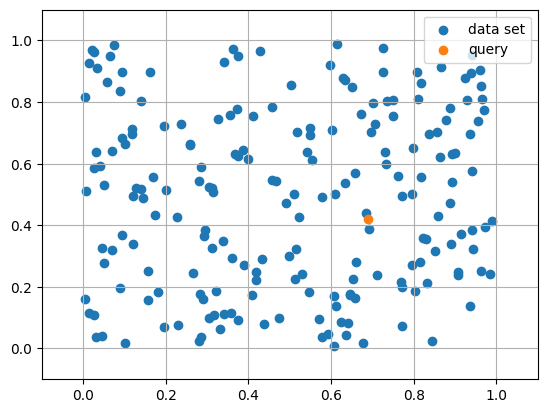
\includegraphics[width=\textwidth]{images/sim-search-init.png}
        \caption{Input of a \(k\)-NNS problem}
    \end{subfigure}
    \hfill
    \begin{subfigure}{0.32\textwidth}
        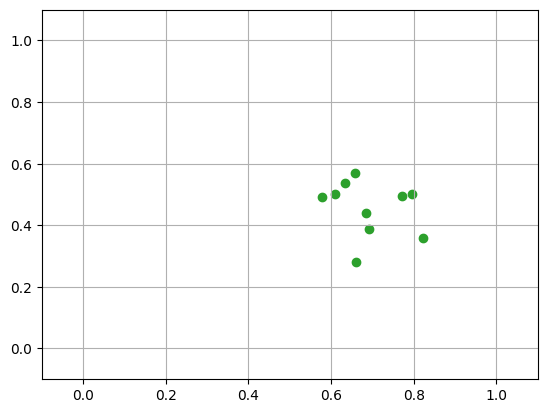
\includegraphics[width=\textwidth]{images/sim-search-knn.png}
        \caption{Output of a \(k\)-NNS problem}
    \end{subfigure}
    \hfill
    \begin{subfigure}{0.32\textwidth}
        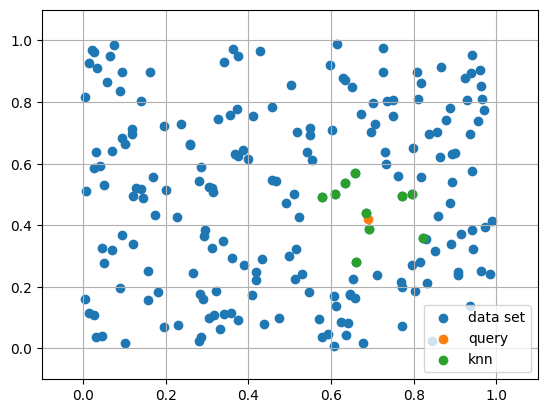
\includegraphics[width=\textwidth]{images/sim-search-final.png}
        \caption{\{In, Out\}put of a \(k\)-NNS problem}
    \end{subfigure}
    \hfill
    \caption{Visualization of \(k\)-NNS in \(\mathbb{R}^2\)}
\end{figure}

\section{ANNS Graphs}

In the real world, big and high-dimensional data sets are becoming more popular. For example, PyThaiNLP converts sentences into 300-dimension vectors that can be used for similarity search. However, finding the exact solutions is often too expensive. Thus, it is more plausible to solve the approximate variant of this problem instead, hence the name \(k\)-Approximate Nearest Neighbors or ANNS, for short. 
Currently, there are multiple approaches used to solve ANNS problems including tree-based \cite{tree-hdindex,tree-optkd}, hash-based \cite{hash-idec,hash-qalsh}, and graph-based \cite{nsg,diskann-paper,hnsw} approaches. However, a recent empirical study \cite{survey2} suggests that graph-based solutions work better especially in higher dimensions due to the curse of dimensionality. So, most recent studies have been focused on designing graph-based data structures that allows for efficient ANNS uses.

Most of the existing studies on ANNS graphs only supports insertion but not removal. This means that if a point or a small portion of the data set becomes stale, it is impossible to remove it. This takes up extra memory or disk space and could also cause queries to return outdated data.
However, removal in ANNS graphs is difficult due to the possibility of the graph becoming disconnected afterwards. This degrades the quality and performance of the graph as a whole. Thus, it is important to design a reconnection method that maintains the quality and performance of the graph after removal.

\section{End Goal}

The short-term goal of this project is to design a data structure that supports efficient vertex removal. However, the ultimate goal of this project is to design an efficient data structure for ANNS in the sliding-window setting due to how uncommon it is looked into in literature (at least at the start of this project).

